\documentclass{beamer}
\usepackage[utf8]{inputenc}
\usepackage{graphicx}
\usepackage{multimedia}
\usepackage{url}

\usetheme{default}
\usecolortheme{crane}
\usefonttheme{default}
\useoutertheme{sidebar}
\useinnertheme[shadow=true]{rounded}

\title{Jeu du Pérudo}
\author{H4104 - Dragibus}
\institute{INSA de Lyon}
% \logo{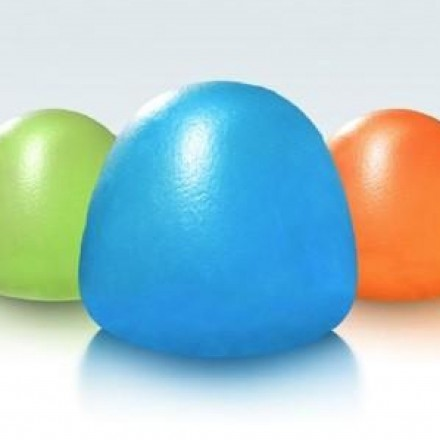
\includegraphics[height=8mm]{logo.jpeg}}

% \AtBeginSection[]
% {
%     \begin{frame}
%     \frametitle{Sommaire}
%     \tableofcontents[currentsection, hideothersubsections]
%     \end{frame}
% }

\begin{document}

\begin{frame}
\titlepage
\end{frame}

\begin{frame}
\frametitle{Sommaire}
\tableofcontents[hideallsubsections]
\end{frame}

\section{Une section}

\subsection{Une subsection}

\begin{frame}
\frametitle{Une frametitle}
Un text.
\uncover<2>{Un texte qui apparait après}
\end{frame}

\subsection{Une deuxième subsection}
\begin{frame}
\frametitle{Un frametitle}
\begin{block}{Un titre de block}
Un texte de block
\end{block}
\end{frame}

\end{document}
